\chapter{Analisis}

\section{Pemilihan Training Data}
Data pada bulan 8 dipilih sebagai training data karena pada bulan tersebut tidak terjadi kerusakan mesin. Disini penulis berasumsi bahwa pada bulan 8 tidak terjadi anomali sama sekali pada data, karena tidak terjadi kerusakan mesin. Namun pada bulan lainnya, walau ada bagian data yang memiliki status mesin NORMAL, bisa saja sebenarnya sudah terjadi anomaly yang menyebabkan machine BROKEN pada hari-hari setelahnya.

\section{LSTM Autoencoder}

Data dipisah menjadi dua bagian, yaitu data normal yang mengandung data dari status NORMAL dan data anomali yang berasal dari status selain NORMAL (BROKEN dan RECOVERY).

Kemudian data dibagi menjadi 3 dataset, yaitu train, validation, dan test. Data train dan validation diambil pada bulan ke-8 awal dan akhir masing-masing dan digunakan untuk training model, sedangkan data test diambil pada selain bulan ke-8 untuk memprediksi hasil anomali.

Proses training model LSTM Autoencoder dilakukan sebanyak 5 epoch yang memakan waktu sekitar 20 menit dengan menggunakan GPU (CUDA). Data train dan validation dibagi menjadi dua macam, yaitu dengan PCA dan tanpa PCA.

Kemudian dilakukan prediksi pada data test dari model yang telah dilakukan training sehingga dapat diperoleh nilai loss yang dihasilkan.

    \subsection{Dengan PCA}

    \begin{figure}[h]
        \centering
        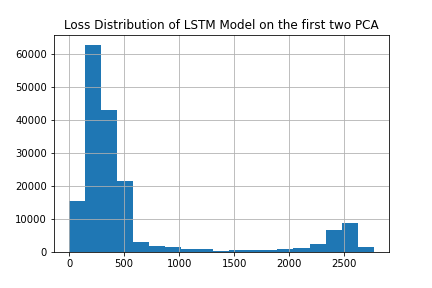
\includegraphics[width=0.6\textwidth]{resources/LSTM/LSTM_PCA_LossDist.png}
        \caption{Distribusi loss LSTM dengan PCA}
    \end{figure}

    Dengan menggunakan nilai threshold 500, diperoleh jumlah data anomali sebagai berikut.

    \begin{table}[h]
        \centering
        \begin{tabular}{|l|r|r|r|}
            \hline
            \multicolumn{1}{|c|}{\textbf{Jenis anomali}} & \multicolumn{1}{c|}{\textbf{Jumlah}} & \multicolumn{1}{c|}{\textbf{Total data}} & \multicolumn{1}{c|}{\textbf{Persentase (\%)}} \\ \hline
            Anomali pada data NORMAL                     & 33866                                & 160430                                   & 21                                       \\ \hline
            Anomali pada data selain NORMAL              & 2237                                 & 14454                                    & 15                                       \\ \hline
        \end{tabular}
    \end{table}

    Jumlah anomali pada data selain NORMAL tidak mencakup keseluruhan total data sehingga terdapat prediksi yang berada pada data dalam kondisi BROKEN atau RECOVERY.

    \subsection{Tanpa PCA}

    \begin{figure}[h]
        \centering
        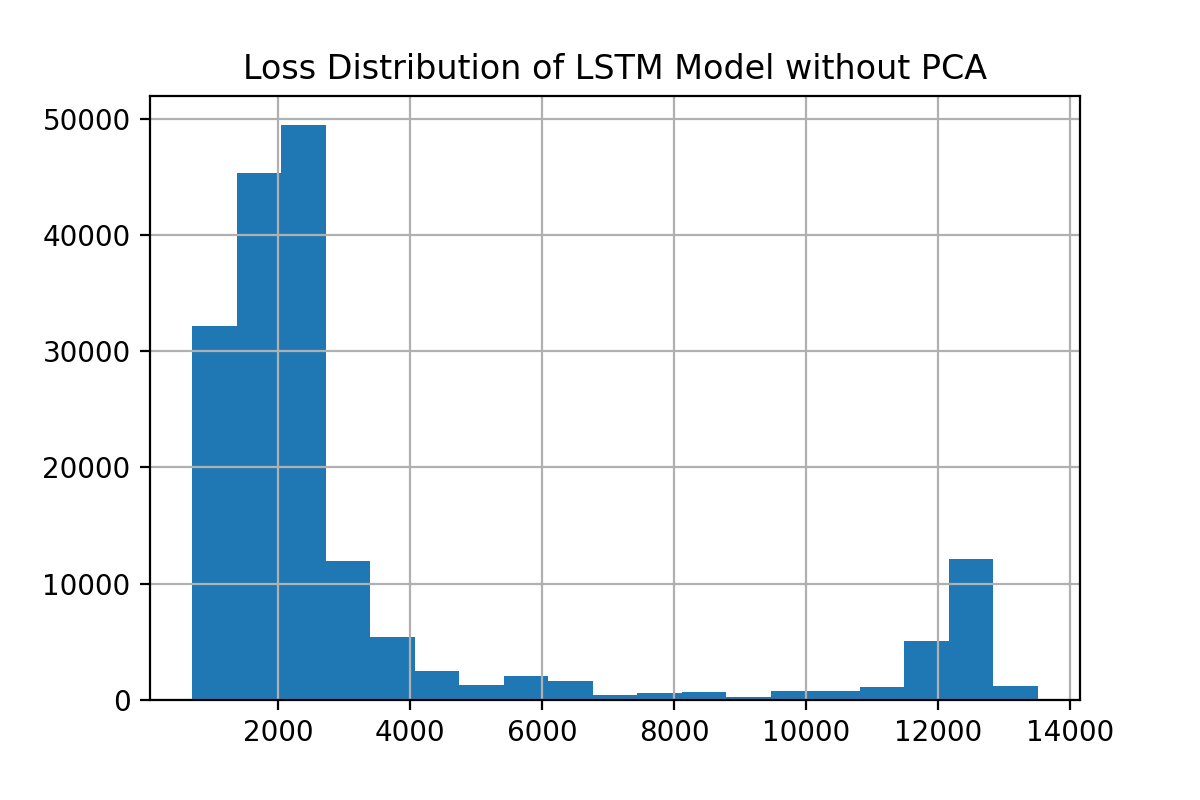
\includegraphics[width=0.6\textwidth]{resources/LSTM/LSTM_noPCA_LossDist.png}
        \caption{Distribusi loss LSTM tanpa PCA}
    \end{figure}

    Dengan menggunakan nilai threshold 3500, diperoleh jumlah data anomali sebagai berikut.

    \begin{table}[h]
        \centering
        \begin{tabular}{|l|r|r|r|}
            \hline
            \multicolumn{1}{|c|}{\textbf{Jenis anomali}} & \multicolumn{1}{c|}{\textbf{Jumlah}} & \multicolumn{1}{c|}{\textbf{Total data}} & \multicolumn{1}{c|}{\textbf{Persentase (\%)}} \\ \hline
            Anomali pada data NORMAL                     & 30182                                & 160430                                   & 19                                       \\ \hline
            Anomali pada data selain NORMAL              & 4979                                 & 14454                                    & 34                                       \\ \hline
        \end{tabular}
    \end{table}

    Terlihat bahwa jumlah anomali pada data NORMAL lebih sedikit 3\% dari analisis dengan PCA, Namun jumlah anomali pada data selain NORMAL juga meningkat hampir 2 kali lipat.

\section{Bayesian Probability}

Data dipisah menjadi training data dan test data. Tidak ada validation data disini, karena validation data digunakan untuk mencegah model overfitting pada training data. Namun karena model bayesian adalah distribusi probabilitas, maka validation data akan menggeser kontur probabilitas dari overfitting pada training data menjadi tepat fit pada training dan validation data sekaligus. Jadi hasilnya tidak akan ada bedanya jika model dilatih pada training dan validation data yang digabungkan. Karena itu, validation data sudah digabungkan kedalam training data, yaitu data pada bulan 8.

Hasil prediksi model Bayesian pada test data menghasilkan distribusi probabilitas data merupakan data normal sebagai berikut.
\begin{figure}[h]
    \centering
    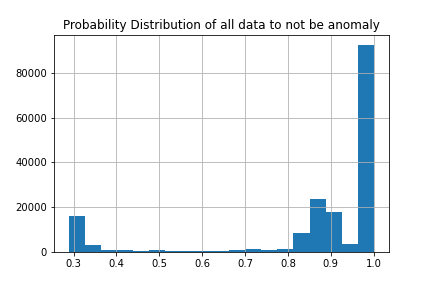
\includegraphics[width=0.8\textwidth]{resources/Bayes/Bayes_ProbDist.png}
    \caption{Prediksi Probabilitas bukan Anomali}
\end{figure}
Kemudian probabilitas tidak terjadi anomali dan terjadi anomali pada tiap waktu sebagai berikut.
\begin{figure}[h]
    %\centering
    \centerline{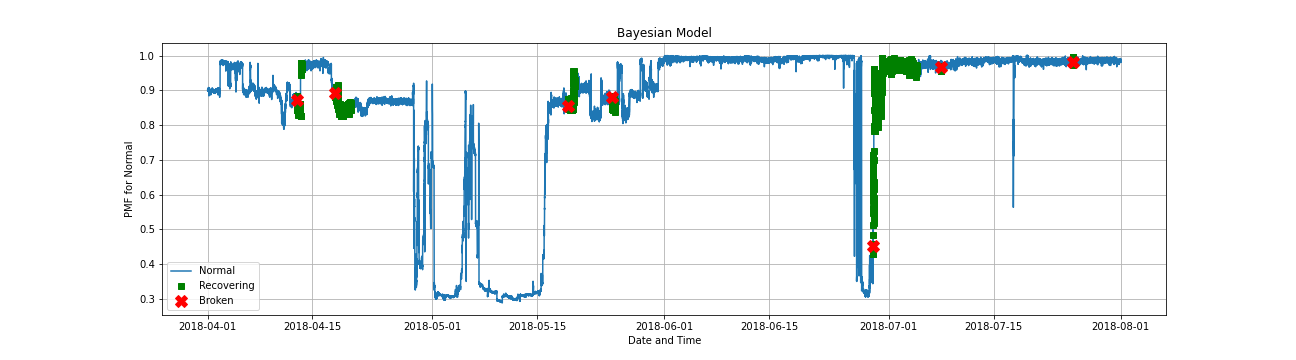
\includegraphics[width=1.4\textwidth]{resources/Bayes/Bayes_normal_PMF.png}}
    \caption{Prediksi Probabilitas bukan Anomali}
\end{figure}
\begin{figure}[h]
    %\centering
    \centerline{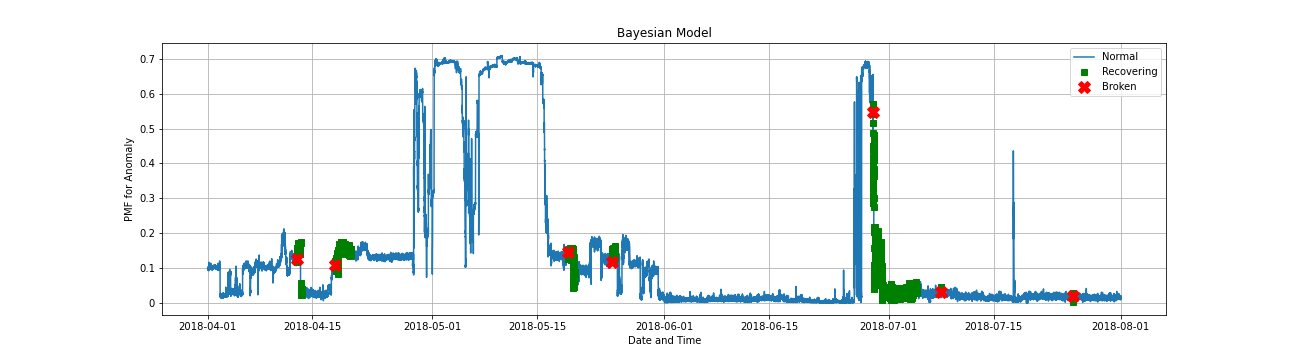
\includegraphics[width=1.4\textwidth]{resources/Bayes/Bayes_anomaly_PMF.png}}
    \caption{Prediksi Probabilitas terjadi Anomali}
\end{figure}
Dengan menetapkan nilai threshold sebesar 0.85, ini berarti jika probabilitas suatu data merupakan data normal dibawah 0.85 sudah ditetapkan sebagai data yang likely merupakan anomaly. Diperoleh jumlah data anomali sebagai berikut.
\begin{table}[h]
    \centering
    \begin{tabular}{|l|r|r|r|}
        \hline
        \multicolumn{1}{|c|}{\textbf{Jenis anomali}} & \multicolumn{1}{c|}{\textbf{Jumlah}} & \multicolumn{1}{c|}{\textbf{Total data}} & \multicolumn{1}{c|}{\textbf{Persentase (\%)}} \\ \hline
        Anomali pada data NORMAL                     & 34527                                & 160430                                   & 22                                       \\ \hline
        Anomali pada data selain NORMAL              & 2567                                 & 14454                                    & 18                                       \\ \hline
    \end{tabular}
\end{table}

\section{Perbandingan Hasil}
Ketiga model memiliki ....

\begin{figure}[h]
    %\centering
    \centerline{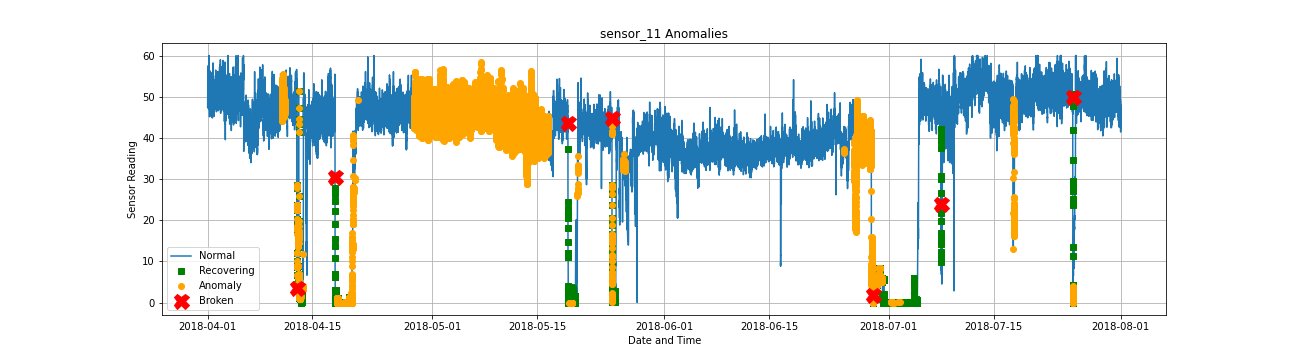
\includegraphics[width=1.4\textwidth]{resources/LSTM/LSTM_noPCA_sensor_11.png}}
    \caption{Hasil deteksi anomali model LSTM tanpa PCA}
\end{figure}
\begin{figure}[h]
    %\centering
    \centerline{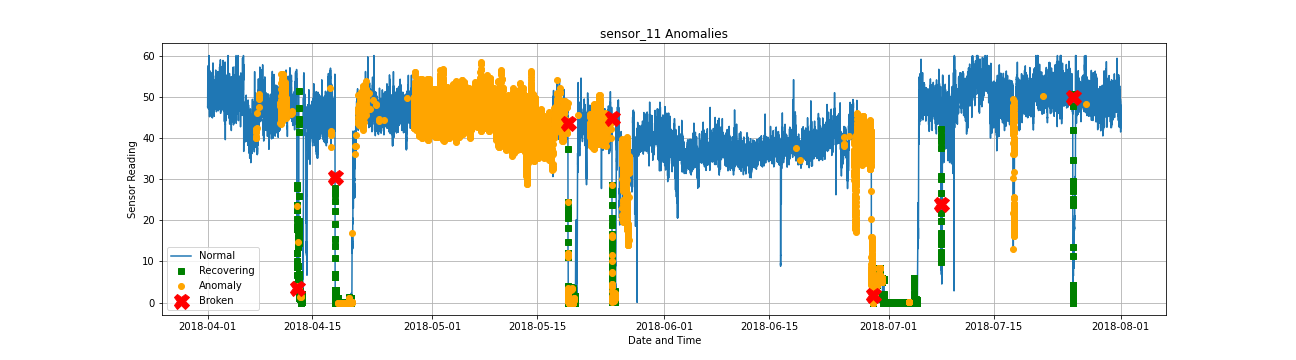
\includegraphics[width=1.4\textwidth]{resources/LSTM/LSTM_PCA_sensor_11.png}}
    \caption{Hasil deteksi anomali model LSTM dengan PCA}
\end{figure}
\begin{figure}[h]
    %\centering
    \centerline{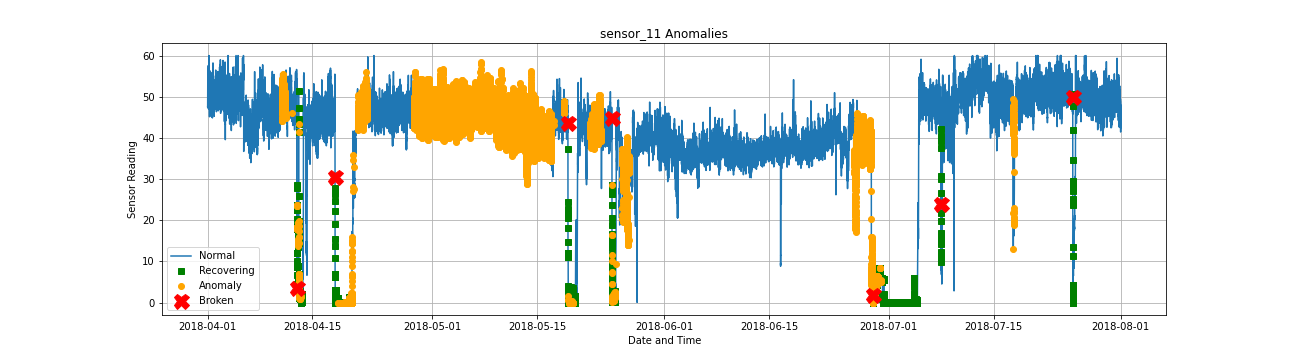
\includegraphics[width=1.4\textwidth]{resources/Bayes/Bayes_sensor_11.png}}
    \caption{Hasil deteksi anomali model Bayesian}
\end{figure}
